\documentclass[12pt]{article}
\usepackage{fullpage,enumitem,amsmath,amssymb,graphicx}
\usepackage{ctex}
\usepackage{multicol}
\usepackage{titlesec}
\usepackage{booktabs}
\usepackage{threeparttable}
\titleformat{\subsubsection}[runin]{\bfseries}{}{}{}[]


\title{贪吃蛇使用说明}
\author{郑立言 \\
	2016011324\\
	 \texttt{zhengly123@outlook.com}\\
	 \texttt{TEL/WeChat:13362756681}}

\begin{document}
  \maketitle
  \rule{\linewidth}{0.4pt}
  
  \textbf{注:程序支持每个房间2至4名玩家,多个房间同时对战。测试中满足了作业要求。}
  \begin{enumerate}
  	
  	
  	\item 打开3个程序
  	\item 其中一个选择合适的端口,点击“Start server”。
  	\item 另外一个程序,点击“Connect to server”。成功后,选择想要的游戏配置,点击"New room"。
  	\item 最后一个程序,填写正确的IP、port,点击“Join room”。
  	\item 游戏中,见图 \ref{fig:inHole} ,可以看到右侧的两个tab,Game tab内,展示了当前游戏状态为正在进行。\textbf{右侧的洞的logo表示,有蛇正在洞中移动,且即将出洞(如果蛇头不在洞中,则不会提示),可能产生危险}。下方的表格显示了各个玩家的生命与积分,以及在线状态。如果玩家离线,游戏将会继续进行。
  	\item 游戏中,可以选择使用方向键与AWSD进行方向控制(由于支持3人及以上的游戏,所有默认所有人都为方向键)。\textbf{按下空格键,可以暂停游戏,Game Status会变为Pause}。如果发起暂停的人,再次按下空格键,则游戏继续进行。
  	
  	\item 游戏中,Music tab可以播放音乐,并可以选择本地歌曲播放。
  	\item 游戏中,右下角为聊天窗口,点击下方的TextField,可以输入信息,回车发送(注意,如果不按回车,则不能操控游戏)。
  	\item 游戏结束后,会弹出龙虎榜,显示历史上得分最高的10个的分。
  	\item 关闭当前窗口,回到步骤3,可以继续下一场游戏。(重复游戏时,请注意房间号码会有变化)。
  	
  	
  	
  	\begin{figure}[h]
  		\centering
  		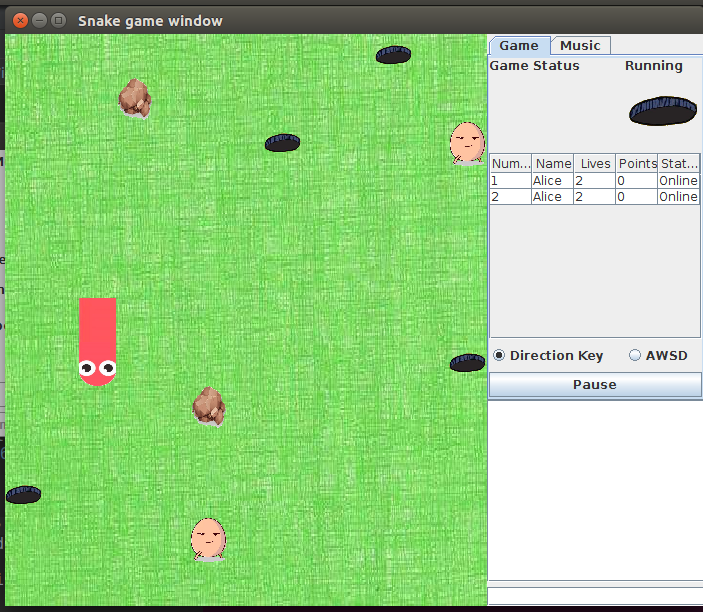
\includegraphics[width=0.7\linewidth]{inHole}
  		\caption{游戏界面}
  		\label{fig:inHole}
  	\end{figure}
  \end{enumerate}
  
\end{document}